\section{Semafori sempre attivo}

Si vuole innanzitutto realizzare una FSM che alterni gli stati come descritto precedente.
Avendo tre stati diversi è necessario impiegare almeno 2 flip-flop: nella nostra implementazione non è stato necessario utilizzarne ulteriori.

Si riporta la codifica scelta in \tab{cod} e lo schema degli stati e delle transizioni in \fig{stati}, dove LV, LG e LR indicano LED verde, giallo e rosso rispettivamente. 

Una tale codifica impone
$$b_{0}^{n+1} =  \overline{b_{1}^{n} \cdot b_{0}^{n}} \qquad \text{e} \qquad b_{1}^{n+1} = b_{0}^{n}$$
in tal modo lo stato indesiderato $00$, non corrispondente a nessuno degli stati codificati, ha comunque una transizione accettabile senza richiedere logica ulteriore.

\begin{figure}[H]
	\begin{minipage}{0.5\textwidth}
		\centering
		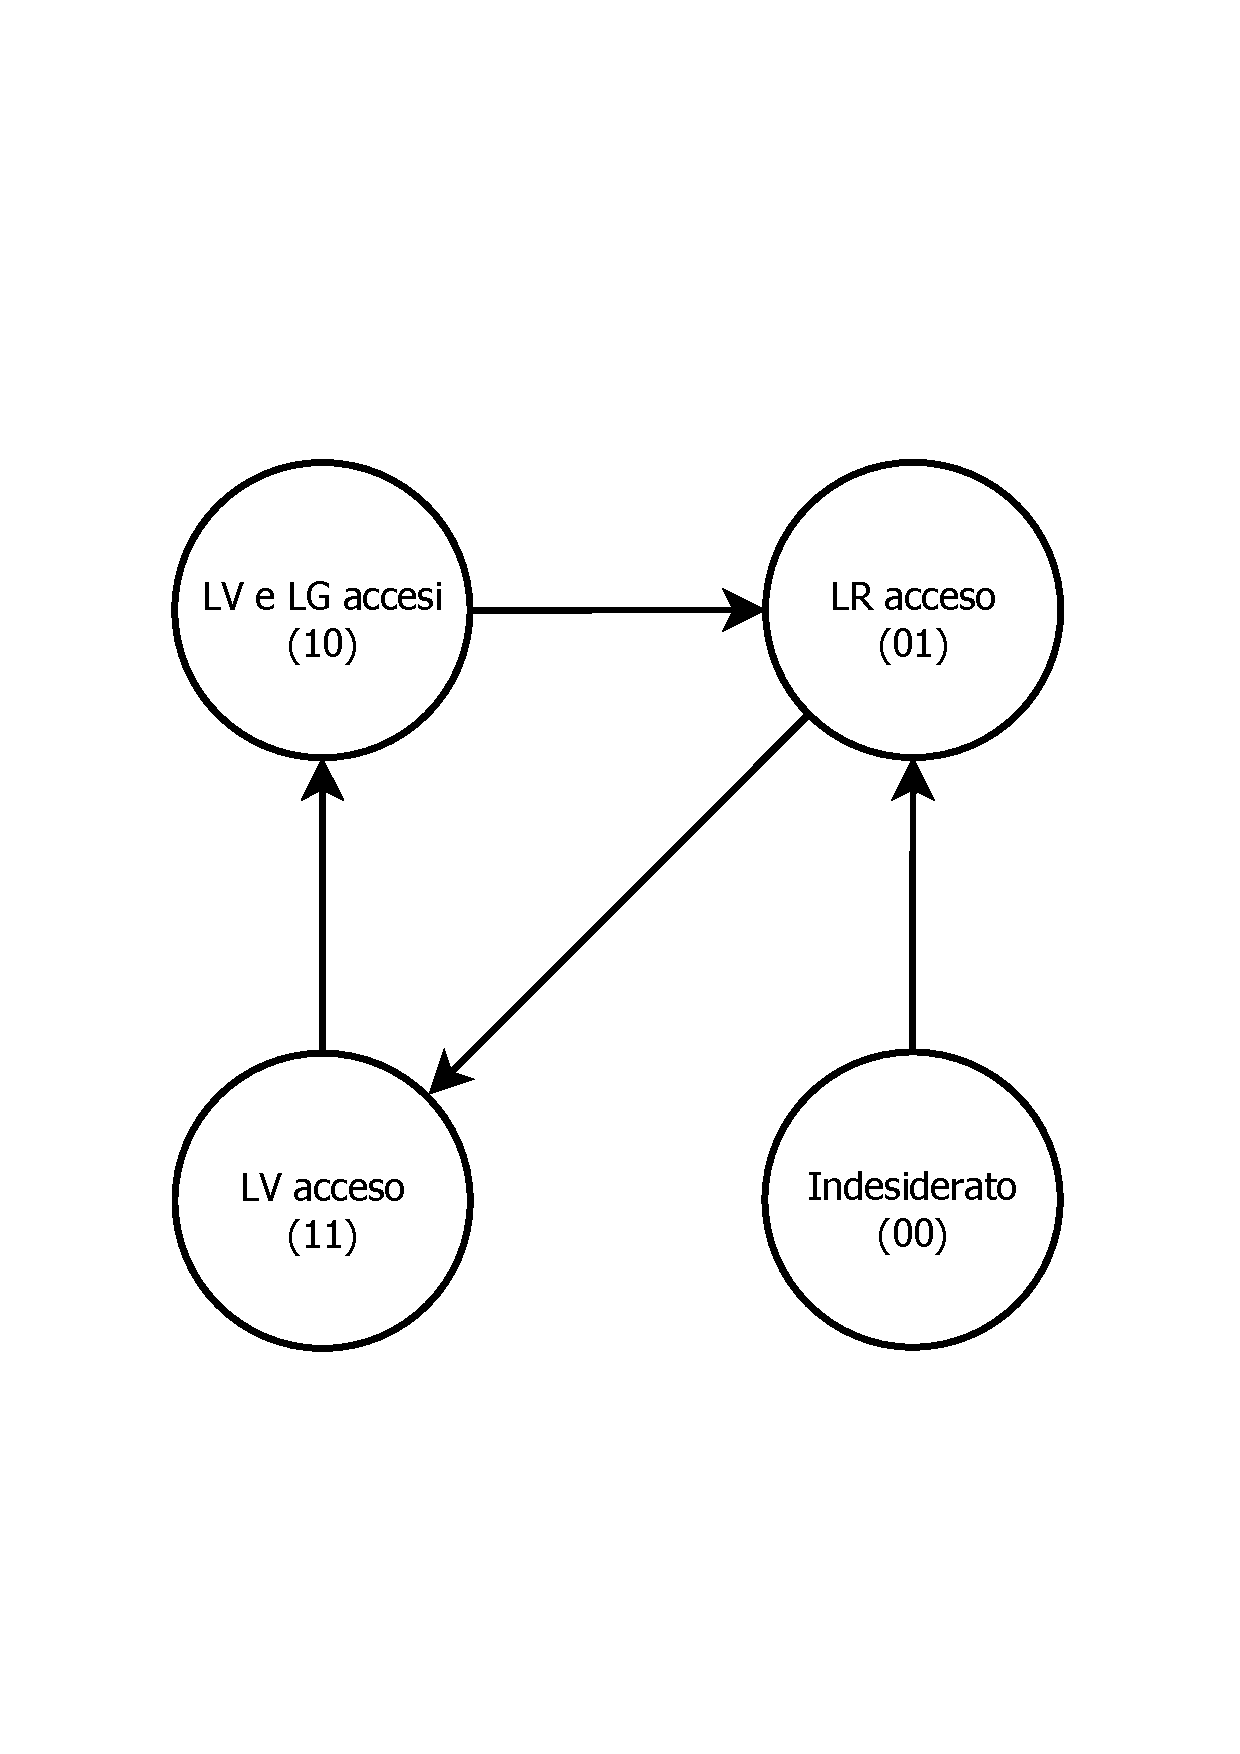
\includegraphics[scale=0.35,trim={0 6cm 0 6cm},clip]{stati_no_enable.pdf}
		\caption{Stati della FSM semaforo senza En.}
		\label{fig:stati}
	\end{minipage}
	\begin{minipage}{0.5\textwidth}
		\centering
		\begin{tabular}{ssc}
			\toprule
			b_1 & b_0 & stato \\
			\midrule
			1 & 1 & verde\\
			1 & 0 & verde \& giallo\\
			0 & 1 & rosso\\
			0 & 0 &  X (indesiderato)\\
			\bottomrule
		\end{tabular}
		\captionof{table}{Codifica degli stati impiegati}
		\label{tab:cod}
	\end{minipage}
\end{figure}

Si riportano in \tablename{ \ref{tab:tran}} le transizioni tra i vari stati della FSM, assieme allo stato desiderato degli output della macchina; tali output sono ottenibili come:
$$LV = b_1 \qquad LG = \overline{b_0} \qquad LR = \overline{b_1}$$

Tali segnali sono ricavabili direttamente agli output $Q$ e $\qbar$ dei D-Latch utilizzati, senza logica aggiuntiva.

La FSM progettata è dunque di Moore, dal momento che l'output dipende solo dallo stato.

\begin{table}[h]
	\centering
	\begin{tabular}{cc|cc|ccc}
		\toprule
		$b_{1}^{n}$ & $b_{0}^{n}$  & $b_{1}^{n+1}$ & $b_{0}^{n+1}$ & \text{verde} & \text{giallo} & \text{rosso} \\
		\midrule
		0 & 0 & 0 & 1  & x (0) & x (1) & x (1) \\
		0 & 1 & 1 & 1  & 0 & 0 & 1  \\
		1 & 1 & 1 & 0  & 1 & 0 & 0 \\
		1 & 0 & 0 & 1  & 1 & 1 & 0 \\
		\bottomrule
	\end{tabular}
	\caption{Tabella delle transizioni della FSM semaforo sempre abilitato; tra parentesi gli output effettivi del nostro circuito per stati indesiderati.}
	\label{tab:tran}
\end{table}

Per realizzare la FSM appena descritta con gli integrati a disposizione è stato realizzato il circuito in \figurename{ \ref{fig:sem2}}. In serie con i LED sono state montate delle resistenze $R\approx 330$ \si{\ohm} per limitare la richiesta di corrente dei LED stessi e tutti gli integrati sono alimentati ad una tensione
$V_{cc}\approx \SI{5}{\volt}$.





\begin{figure}[h!]

	\centering
	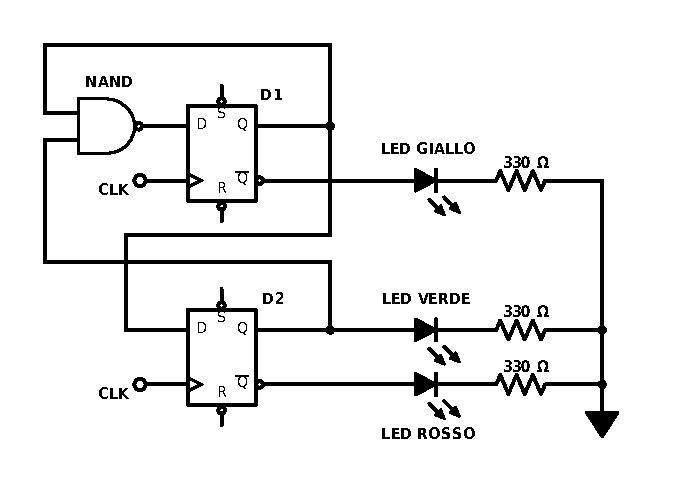
\includegraphics[scale=0.8]{no_enable.pdf}
	\caption{Circuito che realizzi il semaforo senza En.}
	\label{fig:sem2}
\end{figure}

Per la verifica del funzionamento del circuito è stato
inviato un segnale di clock di bassa frequenza ($\sim \SI{1}{\Hz}$) e effettuando un primo controllo osservando l'accensione dei LED. Si è successivamente aumentata la frequenza di clock ($f \sim \SI{170}{\hertz}$) per poter comodamente osservare i segnali all'oscilloscopio e si è acquisito i valori di tensione alle uscite dei vari LED, riportate in
\figurename{ \ref{fig:acq}}. 

\begin{figure}[h]
	\centering
	\subfloat[clock ch1, verde ch2]{
		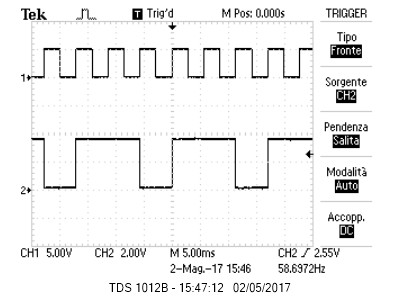
\includegraphics[scale=0.3]{./semaforosemplice/verde.jpg}
	}
	\subfloat[clock ch1, giallo ch2]{
		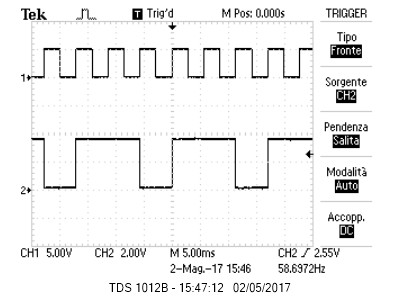
\includegraphics[scale=0.3]{./semaforosemplice/giallo.jpg}
		}
	\subfloat[clock ch1, rosso ch2]{
		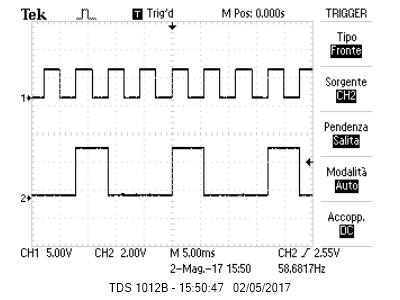
\includegraphics[scale=0.3]{./semaforosemplice/rosso.jpg}
		}
	\subfloat[verde ch1, giallo ch2]{
		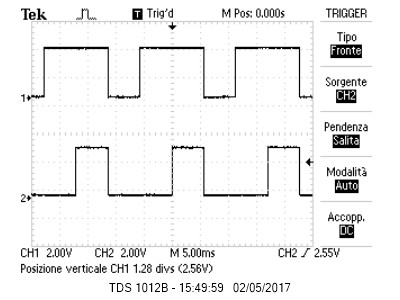
\includegraphics[scale=0.3]{./semaforosemplice/verde_giallo.jpg}
	}
	\subfloat[verde ch1, rosso ch2]{
		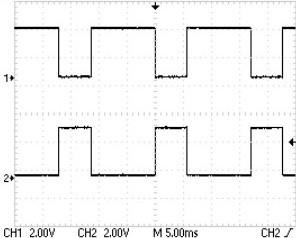
\includegraphics[scale=0.3]{./semaforosemplice/verde_rosso.jpg}
	}\\
	\subfloat[tutti i canali sovrapposti]{
		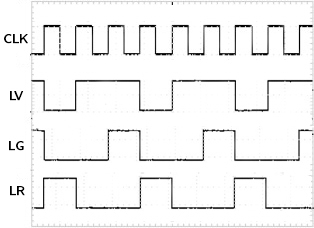
\includegraphics[scale=3]{./semaforosemplice/all.jpg}
	}
\caption{Acquisizione telle tensioni osservate nel semaforo privo di \textit{Enable}}
\label{fig:acq}
\end{figure}
